% Template for ISBI paper; to be used with:
%          spconf.sty  - ICASSP/ICIP LaTeX style file, and
%          IEEEbib.bst - IEEE bibliography style file.
% --------------------------------------------------------------------------
\documentclass{article}
\usepackage{spconf,amsmath,graphicx}
\usepackage{algorithm}
\usepackage[noend]{algpseudocode}
\usepackage{dblfloatfix}    % To enable figures at the bottom of page
\usepackage[svgnames,table]{xcolor}
\usepackage{subcaption,afterpage}
\usepackage[normalem]{ulem}

\newcommand*{\arraycolor}[1]{\protect\leavevmode\color{#1}}
\newcolumntype{A}{>{\columncolor{blue!50!white}}c}
\newcolumntype{B}{>{\columncolor{LightGoldenrod}}c}
\newcolumntype{C}{>{\columncolor{FireBrick!50}}c}
\newcolumntype{D}{>{\columncolor{Gray!42}}c}

% Example definitions.
% --------------------
\def\x{{\mathbf x}}
\def\L{{\cal L}}

% Title.
% ------
\title{Learning Amyloid Pathology Progression from Longitudinal PiB-PET images in Preclinical Alzheimer's disease}
%
% Single address.
% ---------------
\name{Wei Hao$^{1}$ \qquad Nicholas M. Vogt$^{1}$ \qquad Zihang Meng$^{1}$ \qquad Seong Jae Hwang$^{2}$}
\secondlinename{Rebecca L. Koscik$^{1}$ \qquad Sterling C. Johnson$^{1,3}$ \qquad Barbara B. Bendlin$^{1}$ \qquad Vikas Singh$^{1}$}
\address{$^{1}$University of Wisconsin-Madison \qquad
  $^{2}$University of Pittsburgh \\  \qquad $^{3}$William S. Middleton Memorial Veterans Hospital}
%\name{Author(s) Name(s)\thanks{Grant support acknowledgment.}}
%\address{Author Affiliation(s)}
%\address{University of Wisconsin-Madison, Wisconsin Alzheimer's Institute?}
%
% For example:
% ------------
%\address{School\\
%	Department\\
%	Address}
%
% Two addresses (un-comment and modify for two-address case).
% ----------------------------------------------------------
%\twoauthors
%  {A. Author-one, B. Author-two\sthanks{Thanks to ... agency for funding.}}
%	{School A-B\\
%	Department A-B\\
%	Address A-B}
%  {C. Author-three, D. Author-four\sthanks{The fourth author performed the work
%	while at ...}}
%	{School C-D\\
%	Department C-D\\
%	Address C-D}
%
% More than two addresses
% -----------------------
% \name{Author Name$^{\star \dagger}$ \qquad Author Name$^{\star}$ \qquad Author Name$^{\dagger}$}
%
% \address{$^{\star}$ Affiliation Number One \\
%     $^{\dagger}$}Affiliation Number Two
 %
 

 
\begin{document}
\maketitle


%\ninept
%
%
\begin{abstract}
  Amyloid accumulation is acknowledged to be a primary pathological event in Alzheimer's disease (AD).
  The literature suggests that propagation of amyloid occurs along neural pathways as a
  function of the disease process (prion-like transmission), but the pattern of spread
  in the preclinical stages of AD is still poorly understood.
  % While there exist several studies that aim to model the progressive patterns, they often neglect the group-level 
  Previous studies have used diffusion processes to capture amyloid pathology propagation
  using various strategies and shown how future time-points can be predicted at the group level using a
  population-level structural connectivity template. But connectivity could be
  different between 
  distinct subjects, and the current literature is unable to 
  provide estimates of individual-level pathology propagation. 
  We use a trainable network diffusion model that infers the
  propagation dynamics of amyloid pathology, conditioned on an
  individual-level connectivity network. We analyze
  longitudinal amyloid pathology burden 
  in 16 gray matter (GM) regions known to be affected by AD,
  measured using Pittsburgh Compound B (PiB) positron emission tomography at 3 different time points for
  each subject. Experiments show that our model outperforms inference based on group-level trends
  for predicting future time points data (using individual-level connectivity networks).
  For group-level analysis, we find parameter differences (via permutation testing) between
  the models for APOE positive and APOE negative subjects. 

\end{abstract}
%
\begin{keywords}
Alzheimer's disease, Network diffusion, Differential equations, PiB PET image, MRI connectivity
\end{keywords}
%

\section{Introduction}
\label{sec:intro}
Understanding the cause/mechanism of Alzheimer's disease (AD) progression is critical for early treatment and prevention of AD.
Recent neuropathological findings suggest that the progressive pattern of AD could be characterized by the transmission of disease pathologies along neuronal pathways in the brain networks \cite{villain_2008,kuczynski_2010,lo_2010}. 
Specifically, as the “prion-like” disease agents such as misfolded beta amyloid and/or tau protein starts accumulating in the gray matter, the disease pathologies may
\textit{propagate} along the fiber pathways \cite{seeley_2010}.

Motivated in part by these findings, several strategies have been developed to model such propagation patterns using brain imaging data.
% Different models are developed that attempt to capture and thus illustrate the progression patterns.
For instance, the Non-linear neural mass model (NMM) takes the neural activity in localized populations (mini-columns) into account to match with functional connectivity of the brain \cite{honey_sporns_cammoun_gigandet_thiran_meuli_hagmann_2009}.
However, it is a second order state–space differential equation form, so no closed-form solution exists for these formulations and the model construction involves computationally expensive large-scale simulations among the brain signals acquired at thousands of time points.
On the other hand, the Linear network model with a closed-formed solution was formulated as a discretized multivariate auto-regressive linear system for efficiently estimating the brain network signal at different time points \cite{galan_2008}.
Later, the Laplacian of the brain network with physically interpretable parameters was used to model the propagation behavior as a heat diffusion process \cite{raj_kuceyeski_weiner_2012}. 
% because of the lack of group accessible parameters during fitting their models, i.e. there is no group level training process in their models.
Recently, a network diffusion model also used 
a group level Laplacian that captures the group level propagation information of the full cohort to model the propagation of amyloid, a type of AD pathology measurable in PiB PET images  \cite{hwang_ravi_adluru_bendlin_johnson_singh_2018}.
However, the group level Laplacian derived from the model cannot easily
be used to characterize the individual level propagation patterns based on both the baseline imaging scan and the individual's brain connectivity -- propagation routes are based on 
the fiber connectivity of the full group. 
% However, the model suffers when whenever the model is applied on a new subject, the network information that can be derived form its individual Laplacian is lost.

A model which can characterize both the \textit{group level trend}
originating from the underlying disease progression in the full cohort
as well as permit the \textit{individual level variability}
is needed. 
This may enable understanding the pathological progression of AD
not only within the observed timeline but also predict the future disease trends of individuals
at risk of AD -- informed by both the baseline PiB PET imaging scans
and the subject's (structural or functional) connectivity. 
% Essentially, a model that is able to use more information from individual brain network and still reflect the progression pattern on a group level can significantly contribute to the understanding of the pathology of AD, which motivated the work in this paper. 

In this paper, we propose a machine learning 
based model which (1) estimates how to map (via a learned function) 
baseline PiB PET imaging based measurements to measurements 
acquired at a follow-up visit (or even a third visit), 
appropriately informed by the individual's 
connectivity information; 
(2) identifies group level progression similar 
to other important studies \cite{raj_kuceyeski_weiner_2012,hwang_ravi_adluru_bendlin_johnson_singh_2018}
but can offer individual level prediction, 
useful for evaluating risk for 
Alzheimer's disease. 
On the technical side, we formulate a simple
ordinary differential equation that integrates a data-driven heat diffusion equation and a
deep neural network model.
We then evaluate the propagation prediction results on a
neuroimaging dataset and show (promising although preliminary)
group difference results using a genetic risk factor of AD as a dichotomous variable.
% The application of our framework on group analysis between APOE positive and negative subjects suggested the group difference is well developed.

% In summary, our proposed model identifies the diffusive propagation that closely follows the large-scale patterns that many others reported in the aging literature
% % shown consistent with large-scale patterns of disease seen in AD
% \cite{raj_kuceyeski_weiner_2012,hwang_ravi_adluru_bendlin_johnson_singh_2018}, while providing a function which is learnt in the group population, mapping from each individual Laplacian to an altered Laplacian. In this case, this physically realistic model can represent a group trending of the progression patterns along the neorual pathways provided from the structural connectivity without omitting individual network information. The application of our framework on group analysis between APOE positive and negative subjects suggested the group difference is well developed.

\section{Method}
\label{sec:method}

\subsection{MODEL CONSTRUCTION}
\label{ssec:MODEL}

\begin{figure}[!b]
\centering
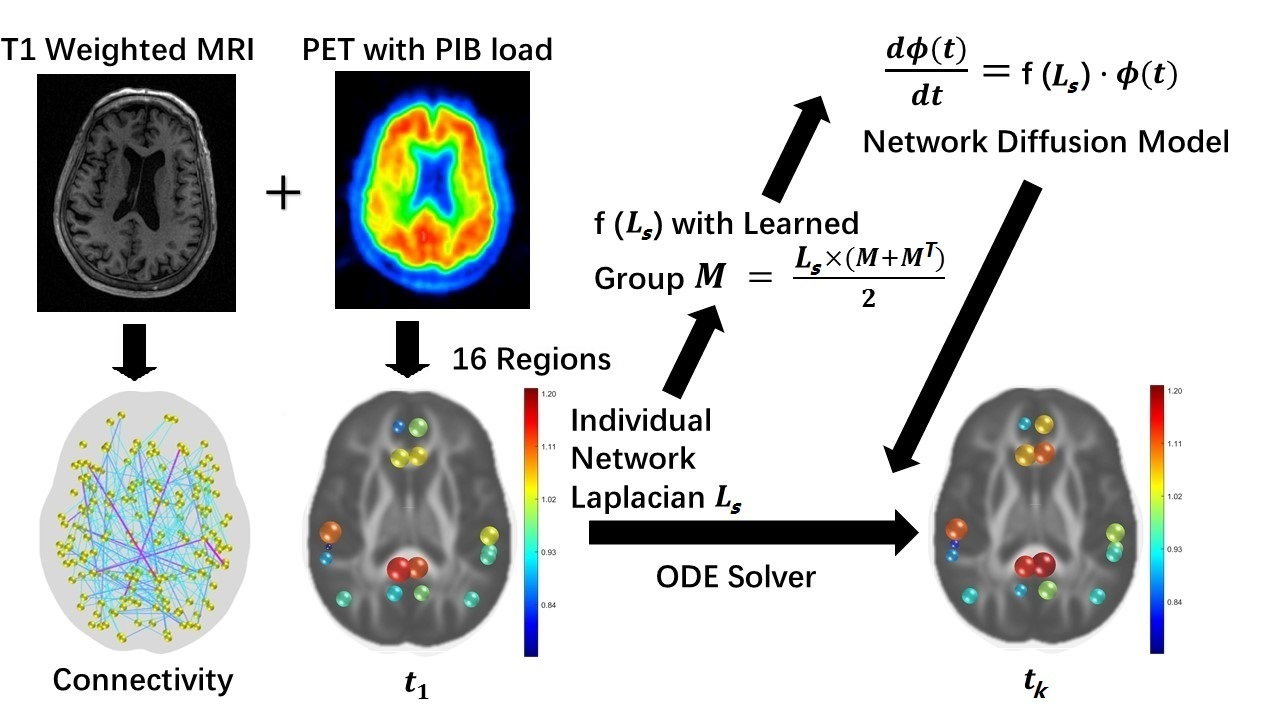
\includegraphics[width=0.935\columnwidth]{we_need_this_TransposeM.jpg}
    \caption{Future time point prediction via a trained model}%
\end{figure}
% As it is mentioned above, Previous studies construct their models using the network diffusion process on a hypothesized 
We construct a brain network roughly similar
to \cite{raj_kuceyeski_weiner_2012} where each connectivity network is denoted as
a graph $G = \{ V,E \}$ of vertices $V$ where node $v_i \in V$ represents the $i$-th
cortical or subcortical gray matter region, and edges $E$ where edge $e_{ij} \in E$ denotes the connectivity 
between $v_i$ and $v_j$. 
Each $e_{ij}$ has a weight $c_{ij}$ denoting the connectivity strength (described in Section \ref{ssec:dataset}). Consider a network which only contains an affected region $R_1$ that is connected with an unaffected region $R_2$. 
Let us denote the level of a measurement 
for the $i$-th region as $\phi_i$. 
Then, the propagation from $R_1$ to $R_2$ will be influenced by 
both the levels $\phi_1$ in $R_1$ and $\phi_2$ in $R_2$ and the inter-region connection strength, $c_{12}$. 
Likewise, we may 
write down the propagation between $R_2$ to $R_1$ assuming a bidirectional connection.
During a period of time $\delta t$, the pathology load in $R_2$ may
increase by $k \cdot (\phi_1 - \phi_2)\cdot \delta t$ where $k$ is a diffusion constant denoting the speed of diffusion. 
As the limit $\delta t \rightarrow 0$, we will have a first-order differential equation:
\begin{equation}
\label{eqn:eq1} 
% \tag{Equation 1}
\frac{d\Phi_{2}}{dt} =k \cdot (\phi_1 - \phi_2)
\end{equation}
Using a Laplacian, we get the \textit{heat diffusion} equation on a network:
\begin{equation}
\label{eqn:eq2}
% \tag{Equation 2}
\frac{d\Phi(t)}{dt} = -k \cdot L \cdot \Phi(t)
\end{equation}

At a time point $t$, $\Phi(t)$ is a vector with the pathology burden measurements
for all regions of interest in an individual's PET scan. Here, $L$ is the graph Laplacian 
constructed with the individual subject's connectivity matrix (see Section \ref{ssec:dataset}). To obtain a propagation pattern
that is consistent across the full training dataset, our model learns a function modulating the diffusion process whose 
start and end points are known when we have longitudinal 
image measurements of the pathology:

\begin{equation}
\label{eqn:eq3}
% \tag{Equation 3}
\frac{d\Phi(t)}{dt} =f(L) \cdot \Phi(t)
\end{equation}

Here, $f$ is the function mapping an subject's $L$, denoted by $L_s$, to $f(L_s)$ through an element-wise product with $\frac{(M + M^T)}{2}$ where $M$ is a matrix of trainable parameters of the same size as the Laplacian and $M^T$ is its transpose:

   \begin{equation}
   \label{eqn:eq4}
%   \tag{Equation 4}
   f(L) = \frac{L \times (M + M^T)}{2}
   \end{equation}
   
This product adjusts the individual Laplacian while keeping it symmetric. Notice that the constant ``$-k$'' is subsumed within $\frac{(M + M^T)}{2}$. Thus, given $\phi(t_1)_s$ and $L_s$ for a subject $s$ at time point $t_1$, $\phi(t_2)_s$ at time point $t_2$ is a solution to an initial value problem by solving this ODE by integration through a differential equation solver \cite{chen2018neural}:

   \begin{equation}
   \label{eqn:eq5}
%   \tag{Equation 5}
   \Phi(t_2) = \Phi(t_1) + \int_{t_1}^{t_2} f(L) \cdot \Phi(t) dt
   \end{equation}
   Finally, our model will be estimated for the entire group of subjects to derive a group level $M$ that
   summarizes how connectivity informs the propagation trend over the entire training data, where the the differential equation denotes the trend. 

\textbf{Training the Model.}
%\label{ssec:train}    
Given $\phi(t_1)_s$, $L_s$ and a {\em integration time} for a subject $s$ at $t_1$,
one can solve the differential equation using standard schemes. 
One issue is that such a mechanism does not easily allow us to backpropagate through the differential equation solver and update the parameters of the function we want to estimate. 
But various strategies have suggested solution schemes, e.g., 
see \cite{chen2018neural}, which yields a differentiable module to produce the predicted ${\hat{\phi}(t_k)_s}$ at
multiple time points $t_k$s.
We trained the model to minimize the $\ell_2$ norm loss between the predicted ${\hat{\phi}(t_k)_s}$ and the corresponding real $\phi(t_k)_s$.
% that the model is fitted on is calculated correspondingly.
Backpropagation on the loss is performed based on the average gradient descent for all training subjects.
The backward algorithm is described in \cite{chen2018neural}.
% {\color{red} Was the backward algorithm mentioned before? Is it for the neural ode?} {\color{green}Back-Propagation will use the backward algorithm in the neural-ode paper}

%{\color{red} Algorithm is here if needed}
\algdef{SE}[DOWHILE]{Do}{doWhile}{\algorithmicdo}[1]{\algorithmicwhile\ #1}%
\begin{algorithm}
  \caption{Training Process}\label{euclid}
          {\small
            \textbf{Input:} \textbf{Model} \eqref{eqn:eq3}; $\phi(t_k)_s$ (DVR data for subject $s$ at time point $t_k$);
            $T$ (artificial integration interval for solving an ODE); $L_s$ (Laplacian for subject $s$);\\
            \textbf{Loss} (the $\ell_2$ norm loss between prediction and real data); 
            \texttt{odesolver} from \cite{chen2018neural}).
            \begin{algorithmic}[1]
              \State \emph{Loop}:
              \If {\textbf{Loss} does not converge}
              \State Initialize \textbf{Loss} to zero for each iteration;
              \State For each subject $s$ in training set, compute prediction ${\hat{\phi(t_k)_s}}$ at time point $t_k$:
              \State ${\hat{\phi(t_k)_s}}=\texttt{odesolve}(\textbf{Model},\phi(t_k)_s,T, L_s)$;
              \State {\em Total Loss} = $\sum_s \|{\hat{\phi(t_k)_s}}, \phi(t_k)_s\|_2$;
              \State Perform average gradient descent on {\em Total Loss} ;
              \State Update group parameter $M$; 
              %\State \textbf{goto} \emph{loop} for next iteration;
              \EndIf
              \State \textbf{close};
            \end{algorithmic}
          }
\end{algorithm}

\begin{figure}[!b]
\centering
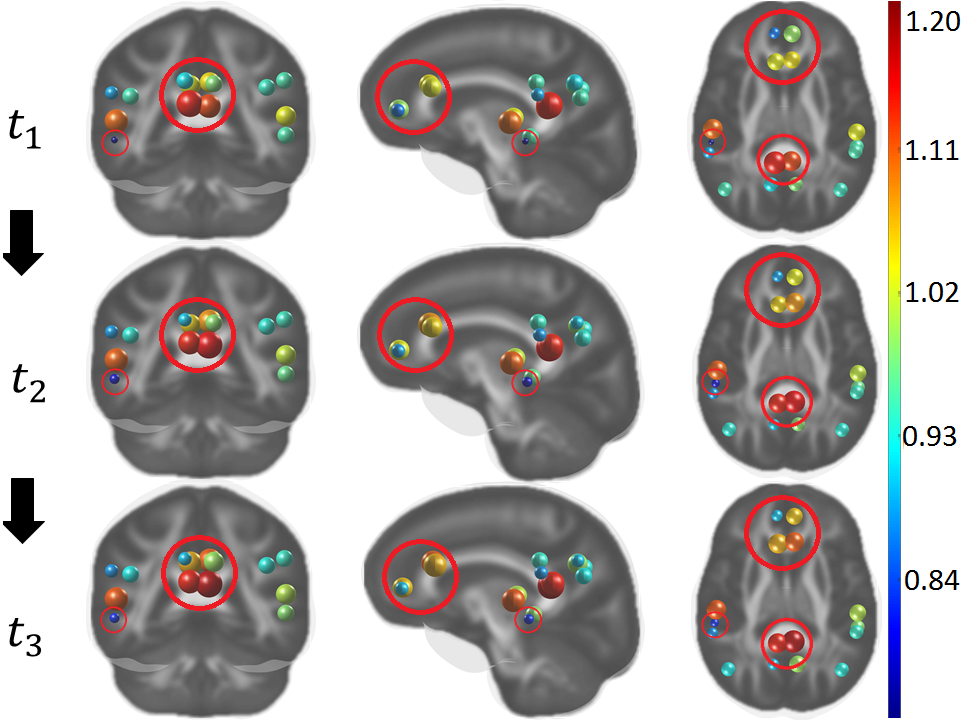
\includegraphics[width=0.7\columnwidth]{brain_fig_circled_longbar.png}
    \caption{Amyloid propagation over time ($t_1 \rightarrow t_2 \rightarrow t_3$)}%
    \label{fig:abstract}
\end{figure}
\section{Experiments}
\label{sec:exp}

\subsection{Dataset}
\label{ssec:dataset}
Neuroimaging data used for these experiments was obtained
from an ongoing large-scale study focused on understanding preclinical Alzheimer's disease (AD). The University of Wisconsin
Health Sciences Institutional Review Board approved all study procedures and all participants provided written informed consent.
Participants who had at least three time points of PiB PET and T1-weighted MRI ($n = 112$, baseline age $67.6 \pm 6.0$ years, $68.6\%$ female)
were included. PiB DVR values were extracted from $16$ regions ($8$ bilateral regions) known to accumulate amyloid pathology \cite{johnson2014amyloid}
and used as regions of interest in the analysis. T1-weighted images were processed using Computational Anatomy Toolbox (CAT12) and `graynet' \cite{raamana2015thickness} 
% (\url{https://raamana.github.io/graynet/})
in order to construct single-subject level connectivity matrices, which provided the strength of connections between the 16 regions.
We used T1-weighted images to keep the initial processing simple -- 
connectivity based on a tractography procedure on diffusion weighted images (DWI) will likely provide better
estimates of connectivity but will need a more involved processing pipeline. 
%due to the fact that not all participants had DWI acquisitions across all time points, and due to changes in DWI acquisition protocols across the study.
Using T1-weighted images allows directly using a common atlas to extract PIB values as well as
calculating connectivity using {\tt graynet} for the same regions without any additional co-registration or tractography.
The single-subject level Laplacian is obtained using graynet estimated connectivity:
\begin{equation}
\label{eqn:eq6}
%   \tag{Equation 6}
L(i,j) = \left\{
\begin{aligned}
-c_{ij} \qquad & \textrm{if  $i \neq j$}&\\ 
%and  $c_{ij}\neq 0$}&\\
 \sum_{(i,j^\prime); e_{ij^\prime} \in E} c_{ij^\prime} \qquad&  \textrm{otherwise}
 %&\\ 0 \qquad & \textrm{otherwise}
\end{aligned}
\right.
\end{equation}
where $c_{ij}$ is the connectivity strength between region $i$ and $j$, and $L(i,j)$ is the entry in row $i$/column $j$ of $L$ for the subject $s$.
Thus, for each subject $s$, we have a $L_s$ (size $16\times16$) for
the baseline time point $t_1$ and three $\Phi_s$ (vectors of size $1\times16$) for three ordered visits. Finally, for group analysis, we use
a well-known AD-related genetic risk factor called APOE \cite{rebeck1993apolipoprotein} as a dichotomous variable, available for 
each
participant in our dataset. We designate participants as APOE+ with a high risk of AD
if they had at least one APOE $\epsilon$4 allele, and APOE- with a low risk of AD if they had no APOE $\epsilon$4 alleles.

\subsection{Experimental Setup and Results}
\label{ssec:split}
We test our model in two scenarios, each with a different dataset split.
% Since we will perform two different experiments, the dataset is split in different settings correspondingly. 
For the first experiment, the model is trained using $\phi(t_1)$, $\phi(t_2)$, and $L$. The training data includes
90\% of the subjects. The model is evaluated on the remaining 10\% subjects to estimate their $\phi(t_2)$ from $\phi(t_1)$ (test).
We perform 10-fold cross-validation. For the second setting, the model is trained using $\phi(t_1)$, $\phi(t_2)$, and $L$ of all subjects
(i.e., scans at $t_3$ are held out). We estimate the accuracy of estimated amyloid loads at $t_3$ (i.e., $\phi(t_3)$) given only
the baseline $\phi(t_1)$.
% while the evaluation is performed on all training subjects,inference their $t_3$ data from their $t_1$ data. 






\textbf{Comparison with inference based on group trends.}
%\label{sec:eval1}
Without knowing the actual PiB DVR values at future time points, a simple evaluation for future PiB DVR estimates obtained
from our model is to compare them to those obtained from using a simple
group-level trend (a linear estimate), i.e., the predicted PiB DVR at time $t_k$ is: 
\begin{equation}
\label{eqn:eq7}
   {\hat{\phi'}(t_k)_s} = \phi(t_1)_s + \frac{\sum_ {s^\prime=1, s^\prime\neq s }^{n} (\phi(t_k)_{s^\prime} - \phi(t_1)_{s^\prime})}{n-1}
\end{equation}
where $n$ is the total number of subjects.

\begin{figure}[!t]
\setlength{\belowcaptionskip}{-0.1cm}
\centering
%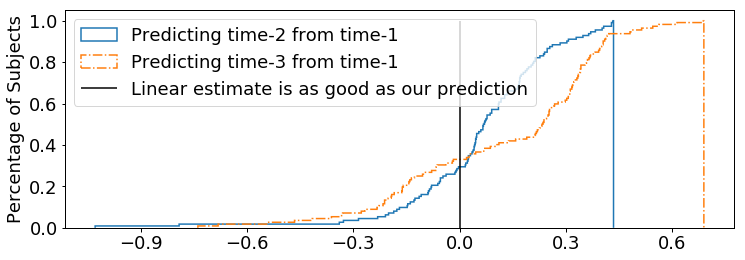
\includegraphics[width=1\columnwidth]{4_new.png}
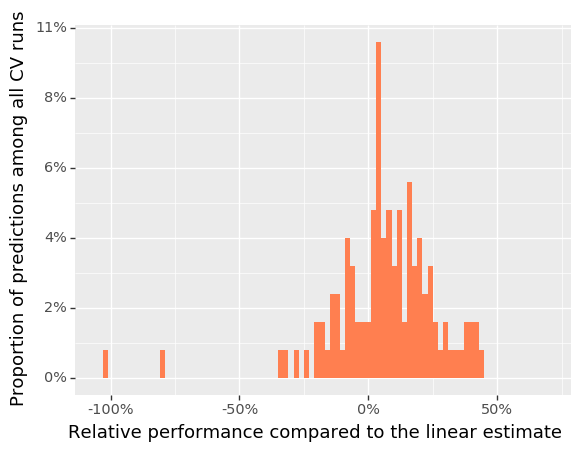
\includegraphics[width=0.495\columnwidth]{4a.png}
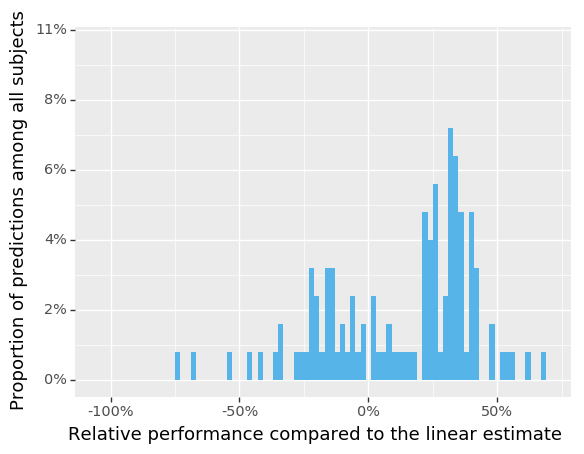
\includegraphics[width=0.495\columnwidth]{4b.png}
\caption{Relative performance w.r.t. the linear estimate of average group change.
  A point on the $x$-axis shows how much better (in percentage) our method is, the $y$-axis shows the frequency.
(Left) predicting $\phi(t_2)$, (Right) predicting $\phi(t_3)$.}%
    \label{fig:BETTER/WORSE}
\end{figure}

\begin{figure}[!t]
\setlength{\belowcaptionskip}{-0.1cm}
\centering
%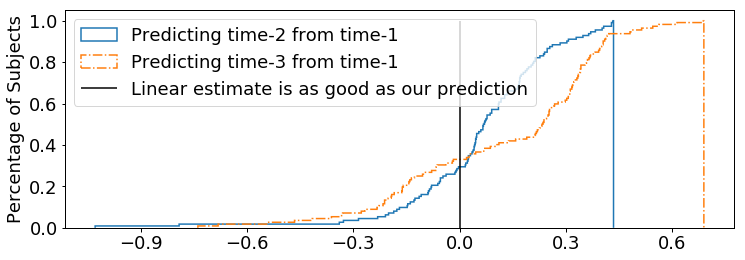
\includegraphics[width=1\columnwidth]{4_new.png}
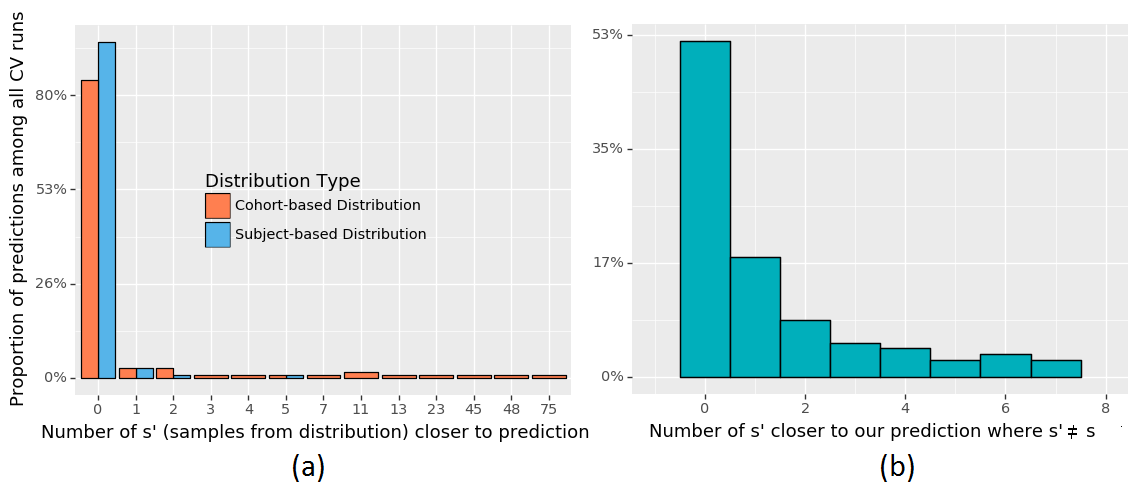
\includegraphics[width=1\columnwidth]{3a_b.png}
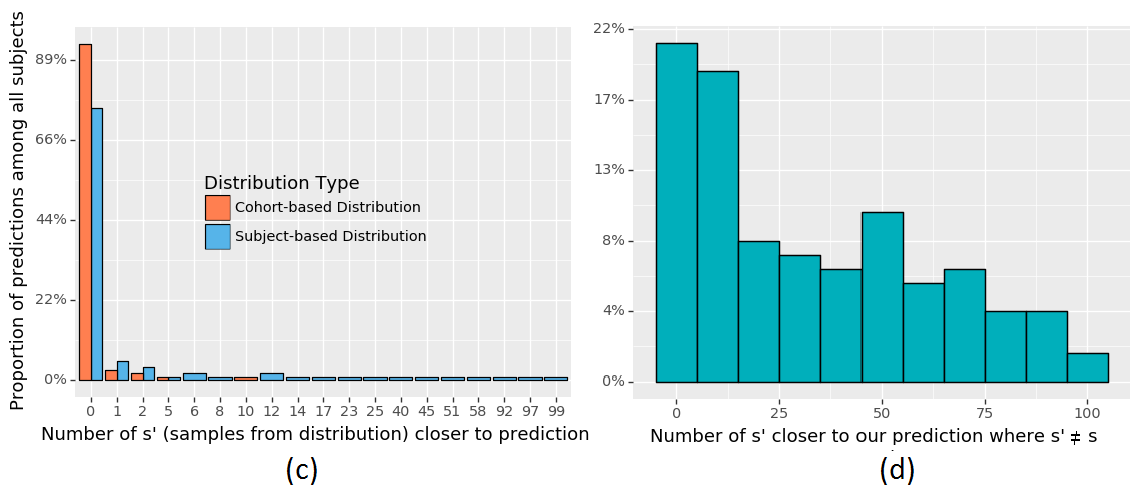
\includegraphics[width=1\columnwidth]{3c_d.png}
\caption{Evaluating if the model's prediction is closest to the amyloid measurements of the correct subject. (Top) predicting $\phi(t_2)$, (Bottom) predicting $\phi(t_3)$.}%
    \label{fig:eval_fig}
\end{figure}

We compare errors in predictions 
from our model (${\hat{\phi}}$) 
versus those made by the linear estimate
(${\hat{\phi'}}$). 
%the percentage of predictions made by our model  %outperforming, evaluated by the loss between %$\phi$), the one made by the baseline  across the %subjects is shown in Table~\ref{tab:group_trend},
The result is plotted as a histogram in Fig. \ref{fig:BETTER/WORSE}.
We found that our model consistently makes better predictions where 70.5\% and 67.0\% are better than the linear estimate
predictions when predicting ${\hat{\phi(t_2)}}$ and ${\hat{\phi(t_3)}}$ using $\phi(t_1)$ respectively.
We also calculated how often (in percentage) relative to the group-level prediction when our model is better (positive value) or worse (negative value) as, 
% by comp The off value and gain value among the worse predictions and better predictions are also calculated respectively:
\begin{equation} % This formulation is kind of weird.Isn't \phi a vector? Does the summation become a percentage? Should j be i? 
\label{eqn:eq8}
    \frac{1}{n}{\sum_ {s=1}^{n} \frac{ \|{\phi(t_k)_s} - {\hat{\phi'}(t_k)_s}\|_2 - \|{\phi(t_k)_s} - {\hat{\phi}(t_k)_s} \|_2}{\|{\phi(t_k)_s} - {\hat{\phi'}(t_k)_s}\|_2}}
\end{equation}
We found that our model captures most of the propagation patterns and performs better
%{\color{red} leave sentence unchanged?}
when we seek to predict DVR measures at $t_3$ when only the baseline scans of each subject are available (average precision gain of
30.1\% and 16.0\% for predicting DVR measures at $t_3$ from $t_1$ and $t_2$ from $t_1$ respectively).



%\begin{table}[!htb]
%\centering
%\begin{tabular}{l|r}
%Evaluation & \% of $\hat{\phi}$ better than $\phi'$\\\hline
%Estimate $\hat{\phi}(t_2)$ from $\phi(t_1)$  & 69.6 \%\\
%Estimate $\hat{\phi}(t_3)$ from $\phi(t_1)$  & 81.3 \%\\
%\end{tabular}
%\caption{\label{tab:group_trend}Prediction Beats Group Trending Addition}

%\label{tab:table1}
%\end{table}

%\begin{table}[!htb]
%\centering
%\begin{tabular}{l|r|r}
%Evaluation &  Better Off&  Worse Off\\\hline
%Estimate t2 from t1 & 14.6 \% & 18.5 \%\\
%Estimate t3 from t1 & 35.5 \% & 43.3 \%\\
%\end{tabular}
%\caption{\label{tab:better/worse_off}Better/Worse Off among  Better/Worse Predictions}
%\label{tab:table2}
%\end{table}





%\subsection{How close is our prediction towards the real data? }
%\label{sec:eval2}
% Among all test subjects, L2 norm is calculated between my prediction of DVR data at $t_ki$ of a subject $ij$ and real DVR data at $t_ki$ for all test data. The expectation is that my prediction for subject $ij$ at $t_ki$ is the closest towards the real DVR data of subject $ij$ at $t_ki$ rather than towards other subjects' data. This evaluation is performed on 10 folds Cross-validation and the result is shown in Fig. 3.(a)  and (b) using the blue line. The x axis of the figure denotes how big the neighborhood of distance is in-between our prediction of a test subject and the real data at that time point for that specific subject. For example, value of 0.2 means that there is one distance of our prediction towards other subject's real data that is smaller than the distance between our prediction of one subject and the real value for that subject if there are 10 distance calculated in total. The y axis denotes the percentage of the subjects in the group. In this sense, the point (0.1,0.8) on the blue line in Fig. 3.(a)  tells us that 80\% of our predictions of a subject is nearly the closest to the real DVR value of that subject among the test population (since we use 11 test data in one folder).   
 
%\subsection{Model prediction vs Random Guess from Test data Distribution}
%\label{sec:eval3} 
%Among all test subjects, L2 norm is calculated between my prediction of DVR data at $t_ki$ of a subject $ij$ and the real DVR data along with 99 randomly generated DVR data at $t_ki$ of that subject. Each random DVR data is generated form the distribution with the mean and standard deviation of the real $\phi_ij$ at $t_ki$. The expectation is that my prediction for subject $ij$ at $t_ki$ is the closest towards the real DVR data of subject $j$ at $t_i$ rather than towards random data. This evaluation is performed on 10 folds Cross-validation and the result is shown in Fig. 3.(a)  and (b) using the orange line. The point (0.09, 1.0) on the orange line in Fig. 3.(a)  tells us that all of our predictions of a subject is the closest to the real DVR value of that subject among the test population.

%A different set of random generated data is calculated for the purpose of the same experiment setting. In this experiment, the data in each region of a randomly generated DVR data at $t_i$ has the distribution with the mean and standard deviation of the real regional data at $t_i$ among the test group. This evaluation is also performed on 10 folds Cross-validation and the result is shown in Fig. 3.(a)  and (b) using the green line. The point (0.09, 0.9) on the green line in Fig. 3.(a)  tells us that 90\% of our predictions of a subject is the closest to the real DVR value of that subject among the test population.

\textbf{How close is our prediction to the real data? }
%\label{sec:eval2}
Among all test subjects, the $\ell_2$-norm is calculated between our prediction $\hat{\phi}(t_k)_s$ and real DVR vector $\phi(t_k)_{s'}$ for
each test subject $s'$. The ideal case is that even if we are slightly off in terms of absolute error in our predictions, nonetheless, this 
 prediction $\hat{\phi}(t_k)_s$ is closer to $\phi(t_k)_s$ relative to other subjects' $\phi(t_k)_{s'}$ ($s' \neq s)$. 
 The results are shown in Fig. \ref{fig:eval_fig}. The $x$ axis denotes how many other subjects $s'\neq s$
 lie between our prediction of measurements for a subject and the real ground truth measurements 
 at that time point for that specific subject $s$.
 %For example, a value of $0$ means that our prediction is the closest to the real data
 %for that specific subject among the whole test group. {\color{red}The $y$ axis denotes the percentage of  subjects in the group}.
 %In this way, the point (0.09,0.71) on the blue trend line in Fig. \ref{fig:eval_fig}(a) tells us that only one {\em other} subject lies between our prediction and the subject of interest for 71\% of our predictions for the test subjects
 %(since we use 11 test subjects in one fold in the cross-validation setting and $\frac{1}{11} \approx 0.09$).
 In Fig. \ref{fig:eval_fig} (b) and (d), we include only the subjects in our test set for this evaluation (for predicting $\phi(t_2)$ and $\phi(t_3)$),
 and find that the model performs well. A simulation experiment is described below. 
 

%\begin{figure*}[!ht]
%  \centering
%    \begin{subfigure}[t]{0.3\textwidth}
%      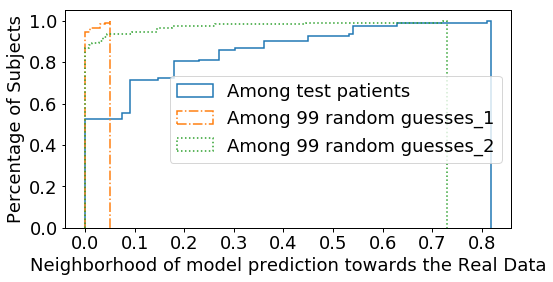
\includegraphics[width=0.9\textwidth]{1.png}
%      \caption{Predicting $\phi(t_2)$ from $\phi(t_1)$}
%    \end{subfigure}
%    \hspace{0.04\linewidth}
%    \begin{subfigure}[t]{0.3\textwidth}
%      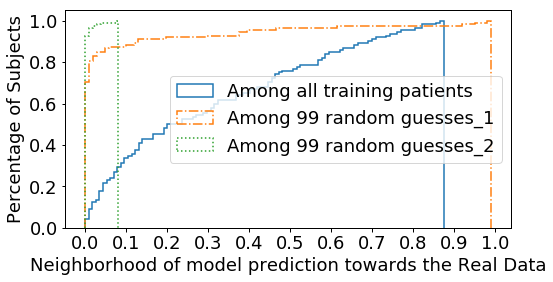
\includegraphics[width=0.9\textwidth]{2_new.png}
%      \caption{Predicting $\phi(t_3)$ from $\phi(t_1)$}
%    \end{subfigure}
%    \hspace{0.04\linewidth}
%    \begin{subfigure}[t]{0.3\textwidth}
%      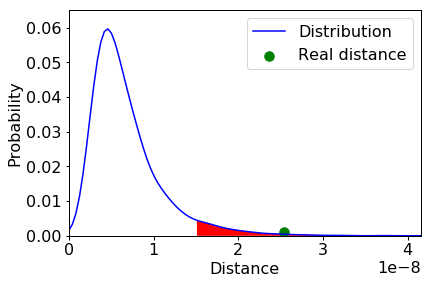
\includegraphics[width=0.7\textwidth]{3.png}
%      \caption{Null hypothesis testing}
%    \end{subfigure}
%    \caption{Evaluation of the model and group analysis}
%    \label{fig:eval_fig}
%\end{figure*}
 
\textbf{Model prediction versus simulated samples from cohort/individual distribution.}
%\label{sec:eval3}
In  Fig. \ref{fig:eval_fig} (a) and (c), we use the cohort distribution or the individual's measurement distribution (orange and blue bars) to artificially ``simulate''
test subjects, again for predicting $\phi(t_2)$ and $\phi(t_3)$. In both cases, we find that the model performs well. 
Among all test subjects, the $\ell_2$ norm is calculated between our prediction $\hat{\phi}(t_k)_s$
and the real DVR vector $\phi(t_k)_s$ along with 99 randomly generated DVR vectors
at that time point $t_k$ of that subject (see Fig. \ref{fig:eval_fig} (a) and (c)). 
Each random DVR vector is generated from the distribution with the mean and standard deviation of the real $\phi(t_k)_s$.
We expect that our prediction $\hat{\phi}(t_k)_s$ is the closest to the real DVR vector $\phi(t_k)_s$ rather than most simulated samples.
Results are shown in Fig. \ref{fig:eval_fig}(a) and (c). We see that 95\% of our predictions for a subject is the closest to the real DVR value
of {\em that} subject.
Next, we assume that the DVR in each region $i$ of a randomly generated DVR vector at $t_k$ for a subject has the distribution
with the mean and standard deviation of the real {\em region-wise} measurements at $t_k$ in the test set such that the DVR data in region $i$ itself,
i.e., $\phi_i(t_k)$, is generated across all $\phi_i(t_k)_s$ for every subject $s$ in the test cohort.
Overall, the model performs well and the results are promising.
%We that 87\% of our predictions for a subject is the closest to the real DVR value of {\em that} subject in the test cohort.



% \begin{figure}[!htb]
%     \centering
%     \subfigure{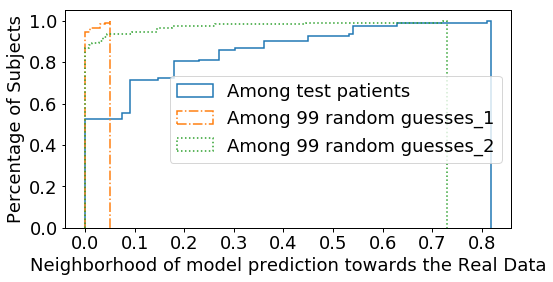
\includegraphics[width=6.5cm]{1.png} }%
%     \caption{Evaluation on Inference t2 Data from t1 Data (remove the grid, remove the white margins, make everything in the figure bigger)}%
%     \label{fig:example}%
% \end{figure}

% \begin{figure}[!htb]
%     \centering
%     \subfigure{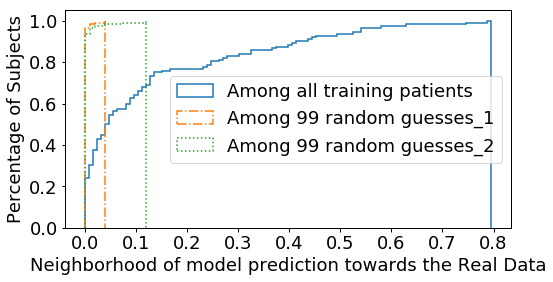
\includegraphics[width=6.5cm]{2.png} }%
%     \caption{Evaluation on Inference t3 Data from t1 Data}%
%     \label{fig:example}%
% \end{figure}

\textbf{Group difference analysis: APOE+ versus APOE-.}
%\label{sec:groupanalysis}
A group analysis is performed between subjects in the APOE positive group ($n = 45$) and APOE negative group ($n = 67$). We split the dataset and train two models, one each for the APOE positive and negative groups, separately. The $\ell_2$ norm between the estimated parameters of the function, $M_1$ and $M_2$ acquired from these two models is computed: this is the statistical summary for the correct group. 
Our null hypothesis $H_0$ is that there is no group level difference between the parameters within these two groups. To test the hypothesis, we also split the dataset randomly but keep the sizes of two groups and calculate the distance between $M$s from the two models within a permutation testing setup. Permutation testing is performed with 10000 draws which gives the null distribution of the summary statistic: difference between the $M$s. The $p$-value is $0.00467$ which is smaller than the significance threshold $\alpha=0.05$ (area plot in red in Fig. \ref{fig:eval_fig}(c)). The null hypothesis is rejected: there is indeed a group difference in terms of the parameters learned by our model to characterize amyloid progression pattern in APOE+ and APOE- groups.

\afterpage{\clearpage}

\section{Conclusions}
\label{sec:conclusion}
%
Recent studies have shown that the early amyloid accumulation patterns may be a strong indicator of AD-related cognitive decline \cite{bilgel2016individual,koscik2019modelingpib}. Our formulation gives 
a mechanism to model amyloid pathology propagation using longitudinal PiB PET imaging data as well as brain connectivity. 
Our model could also serve as a way to estimate the early amyloid accumulation trajectory in the unobserved past (e.g., $t<1$) by ``reversing'' the direction of the process (sign change of $f(L)$), and estimating the start time of 
amyloid accumulation. 
%
%\section*{Acknowledgments}
%\label{sec:Acknowledgments}

{\bf Acknowledgments.} This project was supported in part by RF1 AG059312, R01 AG037639, R01 AG027161, R01 AG021155,
P50 AG033514, UW CPCP (U54AI117924) and NSF CAREER award RI 1252725.



% To start a new column (but not a new page) and help balance the last-page
% column length use \vfill\pagebreak.
% -------------------------------------------------------------------------

%\vfill
%\pagebreak


% References should be produced using the bibtex program from suitable
% BiBTeX files (here: strings, refs, manuals). The IEEEbib.bst bibliography
% style file from IEEE produces unsorted bibliography list.
% -------------------------------------------------------------------------
\bibliographystyle{IEEEbib}
\bibliography{strings,refs}

\end{document}
